\chapter{The Global Signal -- Its Physics and Significance to Cosmology}

\section{Overview of the Epoch of Reionization}
\label{sec:eor-overview}

In brief, the Epoch of Reionization refers to the period of the universe's 
history during which its supply of intergalactic hydrogen became reionized.  
This is important to its evolution, and therefore of interest to astronomers, 
due to the driving factor of that ionization: the ignition of the first stars, 
galaxies, and black holes in the universe. A positive detection of the Epoch of 
Reionization will help astronomers to clarify many open questions of cosmology, 
such as the properties of the first galaxies, how stars with zero metallicity 
formed, the physics of early quasars, and more.

In slightly more detail, let us begin at the beginning. At the start of time, 
the universe was extremely hot and ionized from the Big Bang. Over time, as 
space itself expanded and the gas within the universe cooled adiabatically
at a rate of $T(z) = (1+z)T_0$, the temperature of the universe dropped low 
enough that the nearly-uniform ionized plasma that made up the universe was 
able to recombine to form neutral hydrogen. This phase transition, which 
occurred approximately 380,000 years after the Big Bang at a redshift of $z = 
1098$, enabled photons to decouple from the baryonic matter, thus allowing 
photons to stream freely for the first time in the history of the universe.  
These important periods of the universe's history are aptly referred to as 
``photon decoupling" and ``the surface of last scattering". The surface of last 
scattering also marks the horizon of the observable universe, as everything 
beyond it is simply too opaque to be observable. The radiation released at the 
surface of last scattering, now referred to as the ``Cosmic Microwave 
Background" (CMB), has a mean temperature of $T_0 = 2.725$ K~\citep{fixsen2009} 
and was first observed serendipitously by Arno Penzias and Robert Wilson in 
1964~\citep{penzias-wilson1965}.  

At the point of the CMB, the gravitational force had heretofore always served 
as second fiddle to the electromagnetic force, and the formation of structure 
was driven solely by dark matter~\citep{zaroubi2012}.  As such, structure had 
yet to form, and the release of the CMB led to a period known as the ``Dark 
Ages" -- a time when the universe had nothing to do but slowly get to work 
allowing slight matter over-densities, i.e.~approximately 1 part in $10^5$ more 
dense than the mean density of the universe according to COBE 
observations~\citep{smoot1992}, to grow and transform into stars, galaxies, and 
black holes.

About 100 million years passed and the universe bathed in nothing but the 
after-glow of the Big Bang. Finally, the first galaxies formed, and along with 
them bright stars to emit ionizing radiation. Soon, we find small ionized 
bubbles in the intergalactic medium (IGM), the hydrogen gas filling the space 
between galaxies. Over time, more galaxies and their bright stars make more 
ionized bubbles, until eventually the entire universe's supply of loose 
hydrogen gas has been converted into a proton-electron ionized plasma.

This period, very creatively, is called the Epoch of Reionization -- the epoch 
during which the universe once again became ionized, like it was at the dawn of 
time. As of yet, there has been no confirmed direct detection of the physics of 
this time period -- either of the objects that drive it nor of the gas behavior 
itself.  This has not been for lack of trying. 

For example, EDGES is a small ground-based antenna system in the Murchison 
Radio-astronomy Observatory in Western Australia seeking to detect the 21cm 
reionization global signal directly.  It features two broadband single 
polarization dipole-like blade antennas, one low-band (50-100 MHz) and one 
high-band (90-190 MHz), with a 30x30 m metal ground screen 
below~\citep{monsalve2017}. While there has yet to be a confirmed direct 
detection of the Epoch of Reionization, the EDGES experiment has announced a 
possible detection of the 21 cm reionization global signal~\citep{bowman2018}.

SARAS, similarly, is a 21cm reionization global experiment based in India, 
using a frequency independent fat dipole antenna and a correlation spectrometer 
to measure the average sky temperature across the octave band 87.5-175 
MHz~\citep{patra2013}.  Unlike EDGES, SARAS implements an absorptive ground 
screen rather than a reflective one.

Another tactic to reionization studies is to look for the power spectrum 
signature, rather than the global average phenomena. This is the path taken by 
the PAPER and HERA experiments, both located in the Karoo Desert of South 
Africa and headquartered here in Berkeley, California~\citep{deboer2017}. While 
the power spectrum signal is expected to be fainter than that of the global 
signal, it is also better suited to be observed with a traditional 
interferometer, which relieves some of the fine-tuned calibration concerns that 
plague global signal studies. 

There are many others as well, in all states of existence -- SCI-HI (now 
PRI$^\mathrm{Z}$M) with its distinctive HIbiscus antenna 
design~\citep{voytek2014}, LOFAR attempting to use its general purpose 
instrument in a very specialized way~\citep{rottgering2006}, DARE proposing to 
take the search for cosmic reionization in space itself~\citep{burns2012}. As 
it turns out, these observations are hard to make -- 13 billion light years is 
a long way for light to travel. And that's not even accounting for the blinding 
synchrotron emission from our own galaxy, washing out the reionization signals 
at a scale of 100,000 to 1.

For the sake of brevity and intellectual focus, this thesis (and the experiment 
proposed within) will be focusing solely on observing the overall average 
behavior of the intergalactic medium as it evolves throughout this time period.  
This is referred to as the ``global signal".

\section{Overview of the Global Signal}
\label{sec:global-signal-overview}

The global signal of reionization is an observation of the overall average 
nature of hydrogen throughout this epoch, i.e. the spatially averaged signal 
from the neutral hydrogen gas, as observed using redshifted 21 cm emission from 
the intergalactic medium 13 billion years ago. More specifically, global signal 
experiments seek to observe the relationship between the internal level 
populations of the neutral hydrogen IGM and the ambient temperature of the 
universe, as set by the CMB photons.  This relationship is written 
quantitatively in Eq.~\eqref{eq:21cm-brightness-temp}.

\begin{equation}
    \delta T_b = (T_s - T_\gamma)(1 - e^{-\tau})
    \label{eq:21cm-brightness-temp}
\end{equation}

\noindent where $\delta T_b$ is the observed fluctuation in the 21 cm 
brightness temperature of the 21 cm line ($T_s$) relative to the background CMB 
brightness temperature ($T_\gamma$), and $\tau$ is the optical depth of the 
hydrogen through which the CMB is passing. 

By observing the evolution of the spin temperature relative to the CMB 
background temperature, we are able to better understand how and when energy 
was injected into the gas~\citep{pritchard-loeb2010}. For example, the X-rays 
generated by black holes contributed to the heating of the gas, making the gas 
itself brighter than the ambient photons. Additionally, Lyman-$\alpha$ photons 
from Population II and III stars modify the coupling of the IGM gas temperature 
to the 21 cm spin temperature via the Wouthuysen-Field effect, providing a 
means to track early star formation~\citep{furlanetto2006}.

However, while it's fairly straightforward to observe the 21 cm signal and 
acquire a measurement of the spin temperature through time, that alone doesn't 
give us much insight into the driving physics of that signal. First, we must 
understand what factors contribute to the spin temperature of the gas.

\begin{figure}
    \begin{center}
    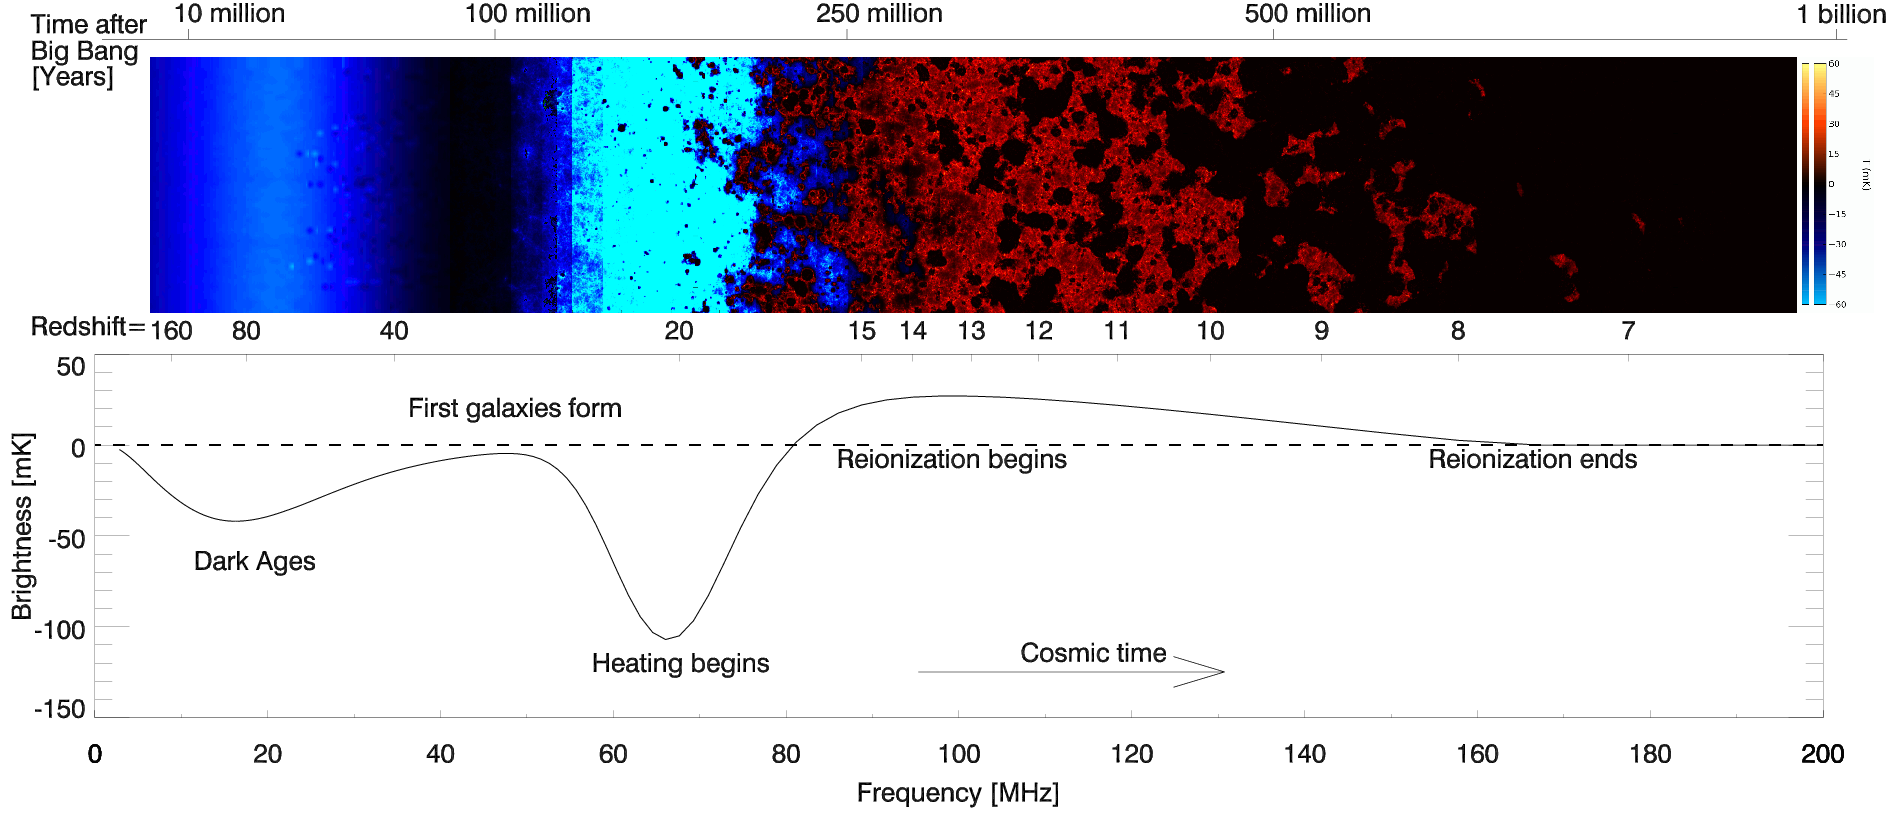
\includegraphics[width=\linewidth]{global_signal.png}
    \end{center}
    \caption{
        In the top half of the figure, we see a cartoon of the reionization 
        history of the universe and the development and growth of ionized 
        bubbles over time. In the bottom half, we see a breakdown of $T_b$, the 
        brightness temperature of the 21 cm global signal, over time. There are 
        five labeled regimes to this plot, each corresponding to the dominance 
        of a different variable in the production of the 21 cm signal. Figure 
        originally published in~\citealp{pritchard-loeb2012}.
    }
    \label{fig:global-signal}
\end{figure}

\subsection{Brief History of the Global Signal}

The most important observable quantity of the global signal, and the one that 
informs us as to the underlying astrophysics at each redshift, is the spin 
temperature $T_s$, which can be described as a weighted average of of the 
ambient CMB photon temperature $T_\gamma$, the kinetic temperature of the 
intergalactic medium $T_K$, the collisional excitation ratio $x_c$, and the 
Lyman-$\alpha$ excitation ratio $x_\alpha$, as shown in 
Eq.~\eqref{eq:spin-temperature}.

\begin{equation}
    T_s^{-1} = \frac{T_\gamma^{-1} + (x_c + x_\alpha) T_K^{-1}}{1 + x_c + 
    x_\alpha}
    \label{eq:spin-temperature}
\end{equation}

The collisional and Lyman-$\alpha$ excitation ratios define the fraction of 
transitions that are being driven by ambient CMB radiation vs. by other 
physical processes (such as collisions or absorption of high energy 
Lyman-$\alpha$ photons),

\begin{equation}
    x_n = \frac{N_{10}}{A_{10}}\frac{T_*}{T_\gamma}
    \label{eq:excitation-ratio}
\end{equation}

where here $N_{10}$ is the excitation rate coefficient of the physical process 
in question (i.e.~the rate at which that particular physical process is driving 
transitions).

Based on these variables, we can define six main physical regimes believed to 
have taken place during the process of structure formation and IGM 
reionization, which can be seen in Fig.~\ref{fig:global-signal} and are 
physically detailed below.

\begin{itemize}
    \item[--] (200 $\leq z \leq$ 1100): During this time period, the residual 
     free electron fraction remaining post-recombination and the high gas 
     density allows the thermal and spin temperatures of the gas to remain 
     coupled with the photon background via Compton scatting and collisional 
     excitations. All temperatures are the same, and therefore there will be no 
     detectable 21 cm signal.
    \item[--] (40 $\leq z \leq$ 200): As cosmological expansion continues, 
     Compton scattering no longer couples the thermal temperature of the gas to 
     the CMB photons, and the gas and radiation decouple and go out of 
     equilibrium.  Collisional coupling sets the spin temperature $T_S < 
     T_\gamma$, leading to an absorption feature in the 21 cm global signal.  
    \item[--] (30 $\leq z \leq$ 40): Expansion continues and collisional 
     interactions are no longer effective at coupling the thermal and spin 
     temperatures of the gas. The excitation levels shift to being set by 
     radiative coupling to the CMB, such that $T_S = T_\gamma$, and there is no 
     detectable 21 cm signal.
    \item[--] (15 $\leq z \leq$ 30): As the first sources (e.g. stars, active 
     galactic nuclei (AGN), etc...) ignite, they begin emitting high energy 
     Lyman-$\alpha$ and X-ray photons. The hyperfine populations couple to the 
     thermal temperature of the cold gas via the Wouthuysen-Field effect, such 
     that $T_S \sim T_K < T_\gamma$, resulting in an absorption feature in the 
     21 cm global signal.
    \item[--] (7 $\leq z \leq$ 15): The radiation (particularly the X-rays) 
     from bright sources heat the gas, $T_K > T_\gamma$ and we see 21 cm 
     emission in the global signal. Lyman-$\alpha$ coupling is still effective 
     at setting the level populations.
    \item[--] ($z \leq$ 7): Enough ionizing radiation has spread throughout the 
     universe that the IGM has been converted from neutral to ionized, and 
     reionization is complete.
\end{itemize}

At present, all redshift ranges listed are theoretical, as no confirmed 
detections have yet been made. However, it is abundantly clear that detection 
and study of this era of this part of the universe's history is rich with 
information about our cosmological origins, and could fill many of the gaps in 
our current knowledge.
